% -*- root: ../main.tex -*-

% Esporre i principali problemi affrontati durante l'effettiva realizzazione delle componenti hardware/software e illustrare le soluzioni implementative adottate. Se l'elaborato ha previsto l'utilizzo di tecnologie già disponibili sul mercato, discuterne brevemente le caratteristiche e motivarne l'adozione rispetto ad altre soluzioni assimilabili. NOTA: in questa sezione devono essere riportate esclusivamente le porzioni di codice ritenute particolarmente significative.

\chapter{Implementazione}
\section{Server}
Per la parte backend ci si è avvalsi della tecnologia Node.js, Express e MongoDb per il database. Per l'invio delle email è stato utilizzato un modulo di Node.js chiamato Nodemailer.


Per supportare la comunicazione bidirezionale tra client e server ci si è avvalsi della libreria Sockets.Io.


Si riportano ora alcuni aspetti implementativi del server che si ritiene opportuno evidenziare. 

\subsection{Forecast e Socket.IO}

All'avvio del Server, viene subito richiamata la funzione di Sockets.IO per rimanere in ascolto di nuove connessioni da parte delle sockets dei clients per richiedere le previsioni meteo:

\begin{lstlisting}[language=Javascript]
io.on("connection", (socket) => {
  socket.on("current", (arg) => {
    if (arg.locality) {
      // Retrieve forecasts by locality.
    } else if (arg.latitude && arg.longitude) {
      // Retrieve forecasts by geolocation position.
    });
    
  socket.on("threedays", (arg) => {
    // Same as before.
  });
});
\end{lstlisting}

In seguito, quando i risultati delle richieste di previsioni meteo ai servizi esterni sono pronti, vengono immediatamente inoltrati ai clients tramite gli eventi delle sockets:

\begin{lstlisting}[language=Javascript]
openWeatherStorage
  .currentByLocation(latitude, longitude)
  .then((result) => {
    socket.emit("result", ...);
  })
  .catch((error) => {
    socket.emit("forecast_error", ...);
  });
  
troposphereStorage
  .currentByLocation(latitude, longitude)
  .then((result) => {
    socket.emit("result", ...);
  })
  .catch((error) => {
    socket.emit("forecast_error", ... );
  });
\end{lstlisting}

\subsection{Autenticazione}

\subsubsection{JSON Web Token JWT}
Per l'autenticazione è stato deciso di utilizzare il sistema JWT (Json Web Token), firmati dal backend. Al momento del login il server rilascia un token al client contenente dei dati utili all’autenticazione. Il client, inviando al server il token ricevuto assieme alle richieste che necessitano di autenticare il richiedente, potrà essere riconosciuto e verificato dal server. In questa maniera il server rimane stateless, dato che le informazioni dell'autenticazione devono essere necessariamente inviate ad ogni richiesta da parte del client.

\begin{lstlisting}[language=Javascript]
// generate token when user log in
userSchema.methods.generateToken = function (cb) {
  var user = this;
  var token = jwt.sign({ _id: user._id }, process.env.SECRET);
  user.token = token;
  user.save(function (err, user) {
    if (err) return cb(err);
    cb(null, user);
  });
};

// find by token
userSchema.statics.findByToken = function (token, cb) {
  var user = this;
  jwt.verify(token, process.env.SECRET, function (err, decode) {
    user.findOne({ _id: decode, token: token },
      function (err, user) {
        if (err) return cb(err);
        cb(null, user);
      }
    );
  });
};

//delete token, when the user logout
userSchema.methods.deleteToken = function (token, cb) {
  var user = this;

  user.update({ $unset: { token: 1 } },
    function (err, user) {
      if (err) return cb(err);
      cb(null, user);
    }
  );
};

\end{lstlisting}

Per facilitare l'utilizzo della validazione del token JWT è stato prodotto un middleware facilmente inseribile nel flusso di Express. Questo middleware recupera il token disponibile dai cookies. Se lo trova associato ad un utente nel database, recupera i dati su di esso e li inserisce nella richiesta per renderli disponibili nell'handler della
route desiderata.

\begin{lstlisting}[language=Javascript]
let auth = (req, res, next) => {
  let token = req.cookies.auth;
  if (!token) {
    // Response the missing token result.
    return res.status(401).json({
      error: "Missing auth token in the request.",
    });
  }

  User.findByToken(token, (err, user) => {
    if (err) throw err;
    if (!user)
      // Notify the unauthorized access.
      return res.status(403).json({
        error: "Didn't found any user matching the auth token provided.",
      });

    // Use the found data in next handler.
    req.token = token;
    req.user = user;
    next();
  });
};
\end{lstlisting}

\subsubsection{Dati sensibili}

Si è avuta la necessità anche di gestire alcuni dati sensibili dell'utente, come le password. E' stato utilizzato bcrypt, un modulo contenente le più comuni funzioni di hashing per salvare le password in maniera sicura
nel database; viene utilizzato al momento della registrazione di un utente
quando si deve salvare la password (viene salvato il suo hash con il
relativo valore di sale), e al login quando bisogna confrontare la password
ricevuta dall’utente con quella salvata.

\begin{lstlisting}[language=Javascript]
userSchema.pre("save", function (next) {
  var user = this;
  if (user.isModified("password")) {
    bcrypt.genSalt(salt, function (err, salt) {
      if (err) return next(err);
      bcrypt.hash(user.password, salt, function (err, hash) {
        if (err) return next(err);
        user.password = hash;
        next();
      });
    });
  } else {
    next();
  }
});

userSchema.methods.comparePassword = function (password, cb) {
  // Compare the user password when user tries to login
  bcrypt.compare(password, this.password, function (err, isMatch) {
    if (err) return cb(next);
    cb(null, isMatch);
  });
};
\end{lstlisting}

\section{Client}
Per lo sviluppo del Client è stato usato Vuetify, un framework di componenti di Material Design per Vue. js che consente agli sviluppatori di creare incredibili applicazioni in modo rapido ed efficiente.

Per gestire lo stato dell'applicazione, abbiamo avuto la necessità di sfruttare il framework Vuex. Esso fornisce un'interfaccia unica per tutta l'applicazione per interrrogare lo stato e modificarlo. Questo permette di avere un'unica fonte di verità dei dati e ne preserva maggiormente l'integrità.

Graficamente potremo delinearne così la struttura:
\begin{figure}[H]
    \caption{Le azioni sono fuori dallo store e diventano servizi}
    \label{fig:Store}
    \centering
    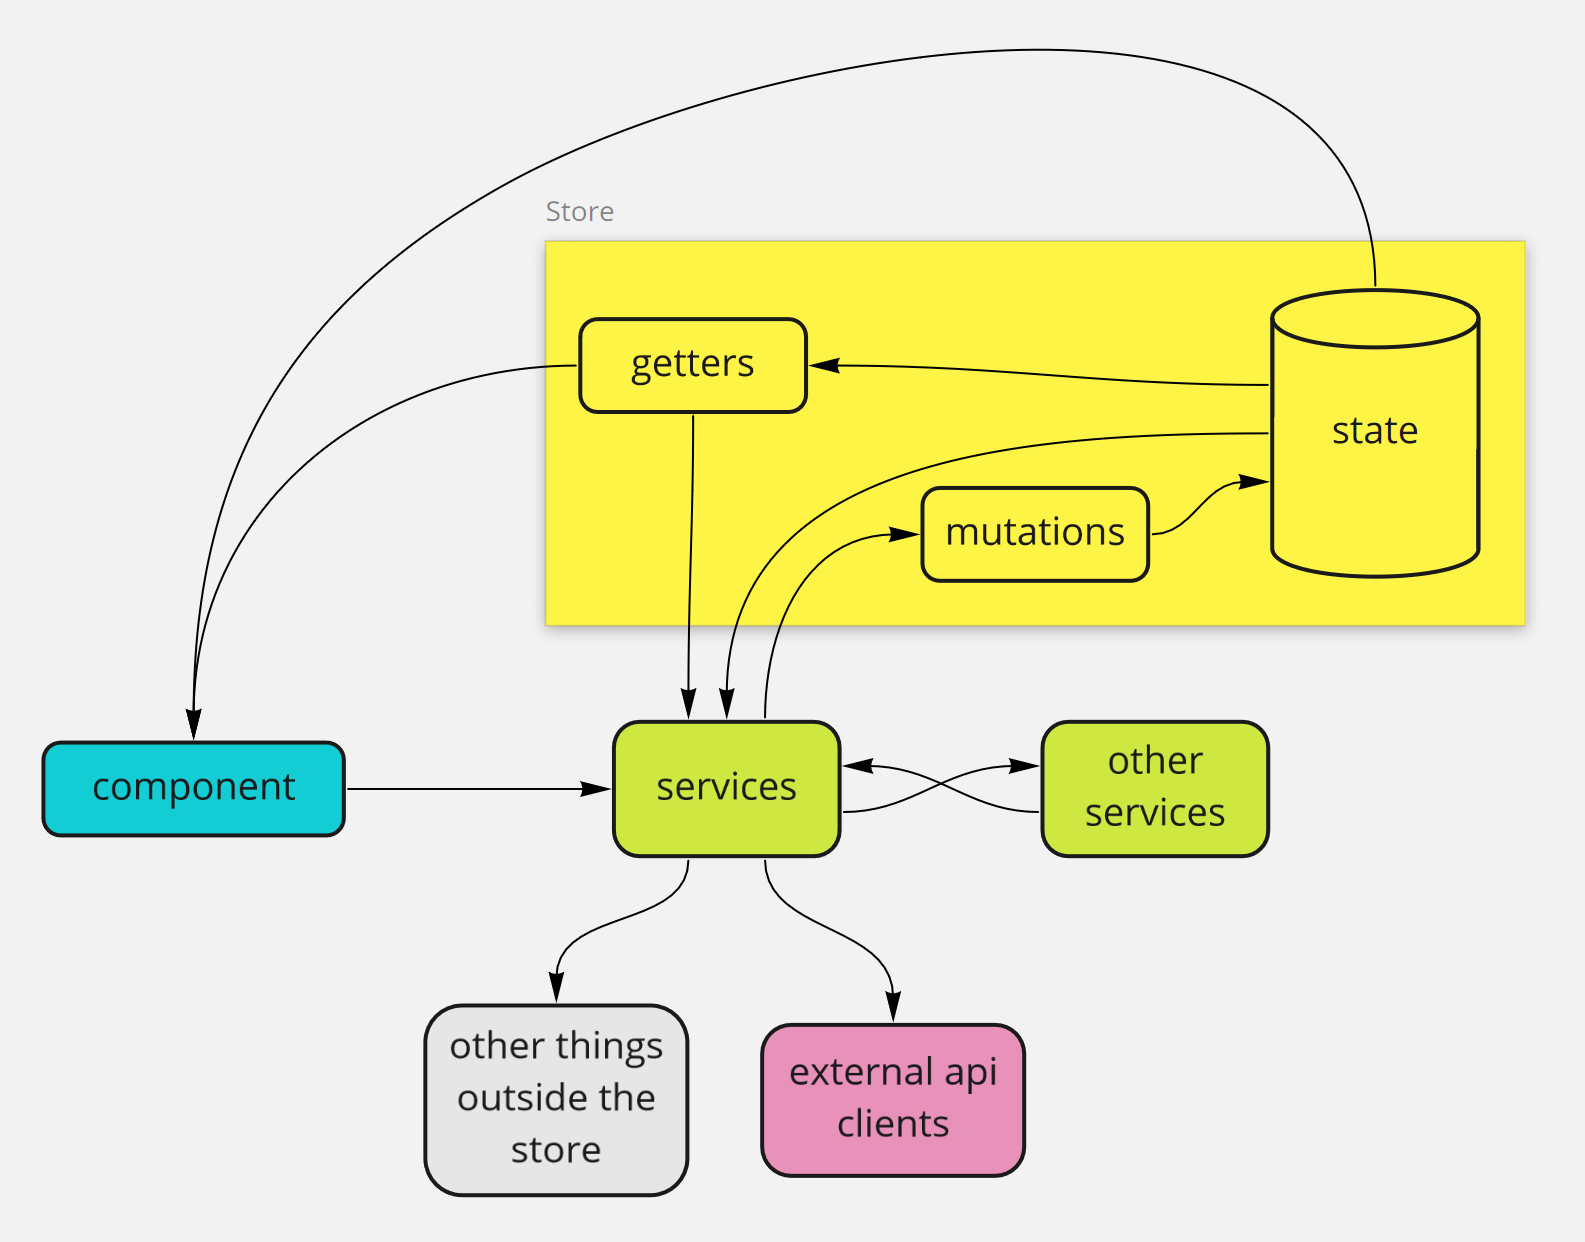
\includegraphics[width=0.7\textwidth]{Images/store.png}
\end{figure}

Il nostro stato è rappresentato dal listato sottostante, in particolare abbiamo memorizzato la visibilità della barra di navigazione e lo stato di autenticazione dell'utente.

\begin{lstlisting}[language=Javascript]
const state = {
  drawer: null,
  user: null,
};
\end{lstlisting}

Lo stato viene quindi letto quando bisogna mostrare o no la barra di navigazione oppure capire quando un utente è autenticato oppure no.

\section{Centralina}
L'applicativo per la centralina è stato sviluppato anch'esso con le tecnologie Node.JS ed Express. Essendo un progetto di simulazione di una centralina reale, dispone di solamente due funzioni: una per ottenere info sullo stato del dispositivo e una per ottenere le condizioni meteo correnti (generate staticamente, data la natura del progetto).

\begin{lstlisting}[language=Javascript]
const express = require("express");
const weather = require("./storage/weather.storage");

const app = express();

app.get("/current", weather.readAll);

app.get("/info", (req, res, next) =>
  res.status(200).json({
    ...
  });
);
\end{lstlisting}

\section{Prodotto Finale}
\label{prodottofinale}
Il prodotto finale ha subito delle evoluzioni rispetto al \href{https://github.com/Weather-Vortex/WeatherVortex-Report/raw/main/MockUps/WeatherVortex-Mockup.pdf}{mockup} ma segue comunque le linee
guida imposte. Nonostante la resa grafica sia stata rivoluzionata, la user experience e i meccanismi di navigazione del sito sono rimasti gli stessi.  Il cambiamento più degno di nota è stato lo spostare le voci del menù dalla barra in alto all'apposito scomparto a sinistra. Qui di seguito sono riportati gli screenshot delle schermate più importanti.

\begin{figure}[H]
    \caption{Pagina Home finale}
    \label{fig:imHome}
    \centering
    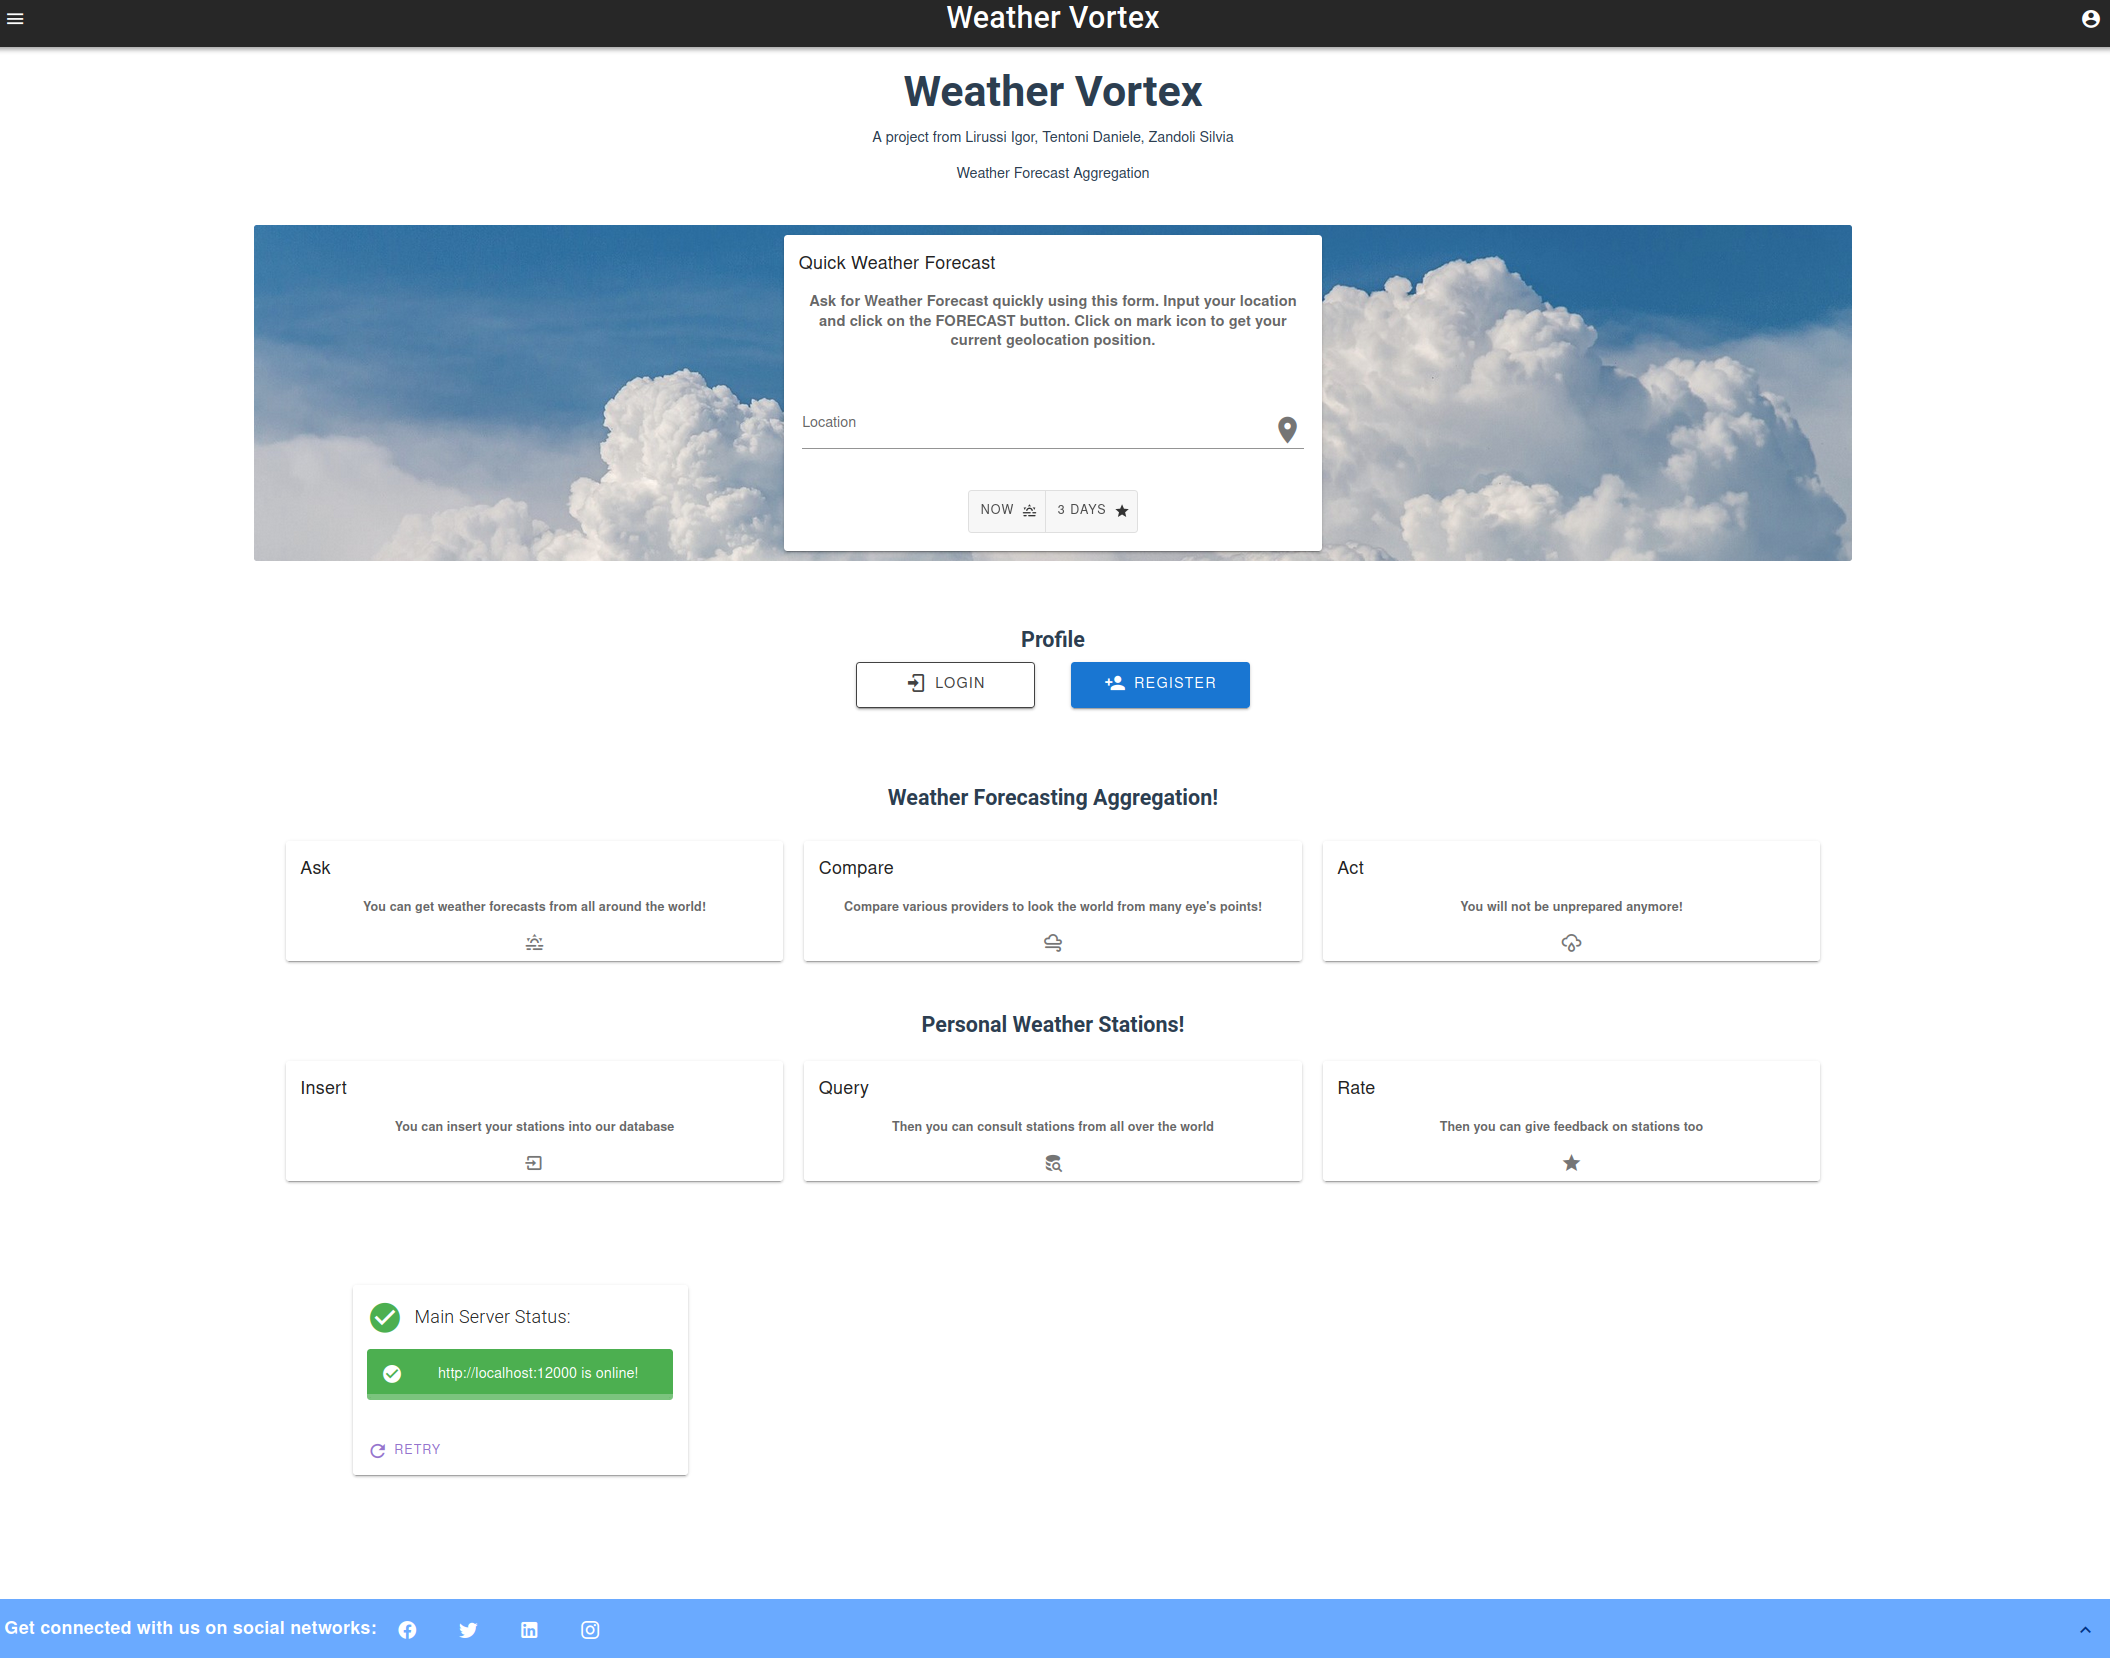
\includegraphics[width=1\textwidth]{Images/homepage.PNG}
\end{figure}
La home del sito è la pagina visivamente più importante, in quanto sarà la prima che l'utente visualizza e quella che vedrà più spesso. Per facilitare l'esperienza, il primo box disponibile è quello delle previsioni. Questa scelta è stata fatta soprattutto per incentivare i nuovi utenti a provare le funzionalità del sito immediatamente, senza che debbano sforzarsi a cercarle. Oltre all'immediatezza intuitiva la scelta aiuta a velocizzare le operazioni per i visitatori assidui del sito, che vogliono raggiungere il risultato desiderato con il minore numero di click possibili.

Sotto all'elemento per le previsioni sono disposti due pulsanti di Login e Registrazione. Questo funge da incentivo a creare un account o a effettuarvici l'accesso. Qualora l'utente effettui il login e ritorni sulla home, i pulsanti non saranno più visualizzati.

\begin{figure}[H]
    \caption{Pagina Login finale}
    \label{fig:imLogin}
    \centering
    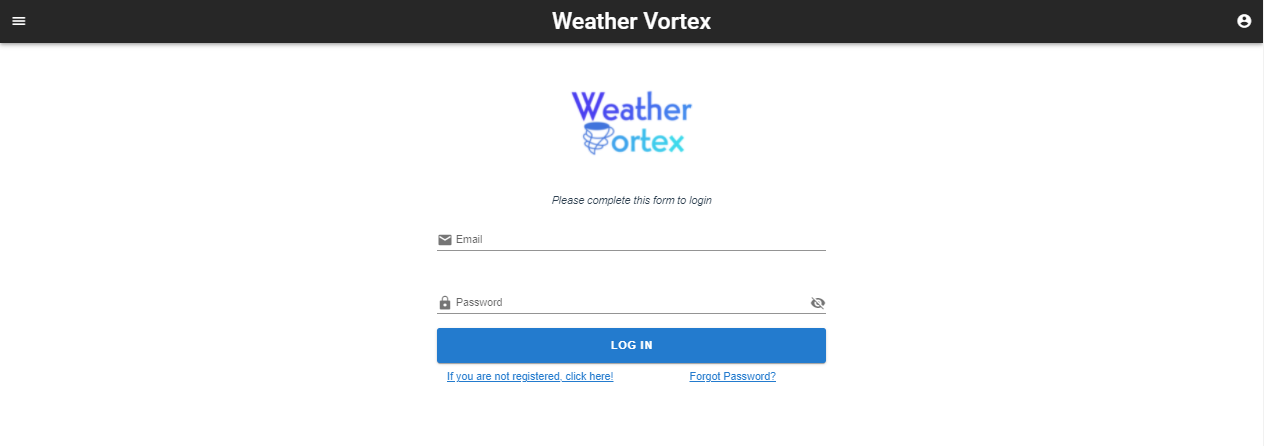
\includegraphics[width=1\textwidth]{Images/Login1.PNG}
\end{figure}
La schermata di login ha una resa molto funzionale e chiara. Questa scelta ha lo scopo di rendere semplice e intuitiva l'operazione chiave di collegarsi al proprio account, senza che l'utente possa cliccare altrove e non portarla a termine.
 
\begin{figure}[H]
    \caption{Pagina Profilo Privato finale}
    \label{fig:PrivProf}
    \centering
    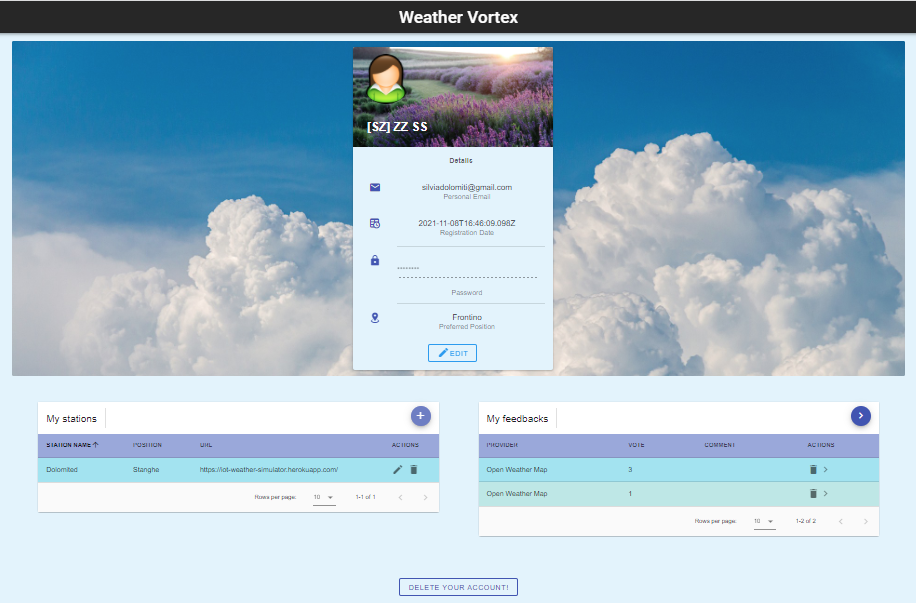
\includegraphics[width=1\textwidth]{Images/PrivateProfile.PNG}
\end{figure}
Il profilo privato permette di gestire i propri dati. Un design tabulare è stato scelto per rendere chiare le varie operazioni possibili di modifica e cancellazione. Tramite le due tabelle l'utente può visionare immediatamente i feedback rilasciati e quali centraline siano collegate al suo profilo. 

\begin{figure}[H]
    \caption{Pagina Previsioni finale}
    \label{fig:imForecast}
    \centering
    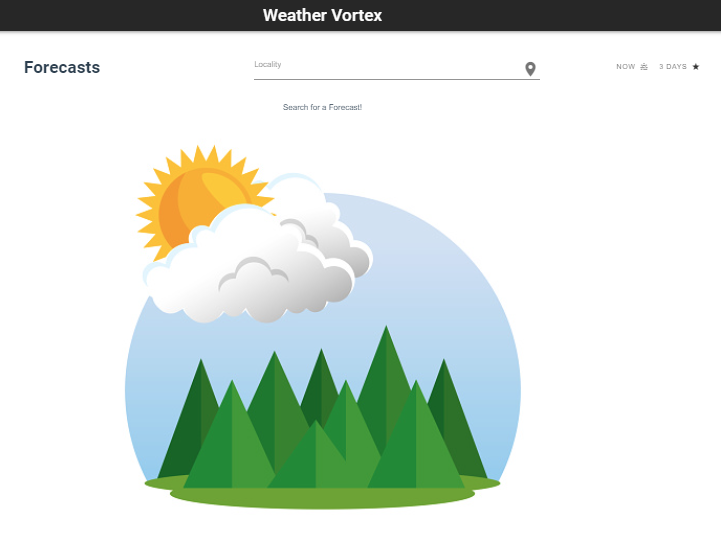
\includegraphics[width=1\textwidth]{Images/ForecastIn.PNG}
\end{figure}
La pagina delle previsioni permette di selezionare una posizione e scegliere tra la previsione corrente e quella futura fino a 3 giorni. Nella barra di ricerca è possibile scrivere il nome di una località o passare direttamente le coordinate. Qualora si volesse avere le previsioni nella posizione corrente è possibile chiedere la geolocalizzazione.

La pagina delle previsioni attuali permette di comparare facilmente le differenti previsioni dei provider. In alto è disponibile sempre la barra di ricerca geografica per cambiare località. 
Un'ulteriore barra di ricerca fornisce la possibilità di ricercare uno specifico provider o centralina digitando il nome o parte di esso.

La card centrale fornisce i dati aggregati.  La stima viene fatta prendendo la media dei valori e la previsione con frequenza maggiore.

\begin{figure}[H]
    \caption{Pagina Previsioni attuali finale}
    \label{fig:imForecast1}
    \centering
    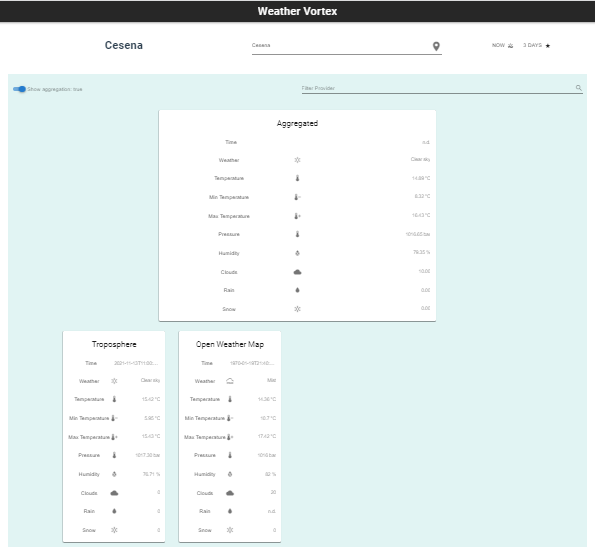
\includegraphics[width=1\textwidth]{Images/Forecast3.PNG}
\end{figure}

\begin{figure}[H]
    \caption{Pagina Previsioni per tre giorni finale}
    \label{fig:imForecast2}
    \centering
    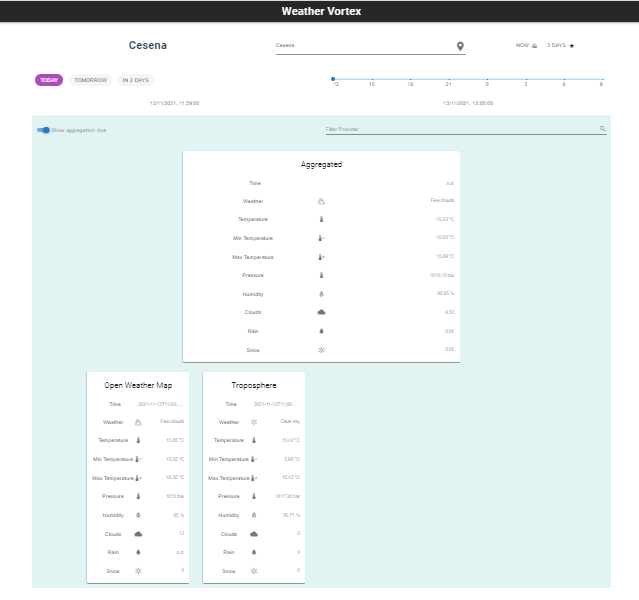
\includegraphics[width=1\textwidth]{Images/Forecast3days.PNG}
\end{figure}
La pagina con le previsioni future segue lo stesso schema della pagina delle previsioni attuali. La scelta è stata presa per facilitare l'utente per permettergli di decidere di scegliere la finestra temporale di cui sapere le previsioni. Inoltre, sono presenti dei pulsanti per poter selezionare le 3 giornate successive e uno slider per poter decidere anche l'orario.

\begin{figure}[H]
    \caption{Pagina Feedback finale}
    \label{fig:imFeedbacks}
    \centering
    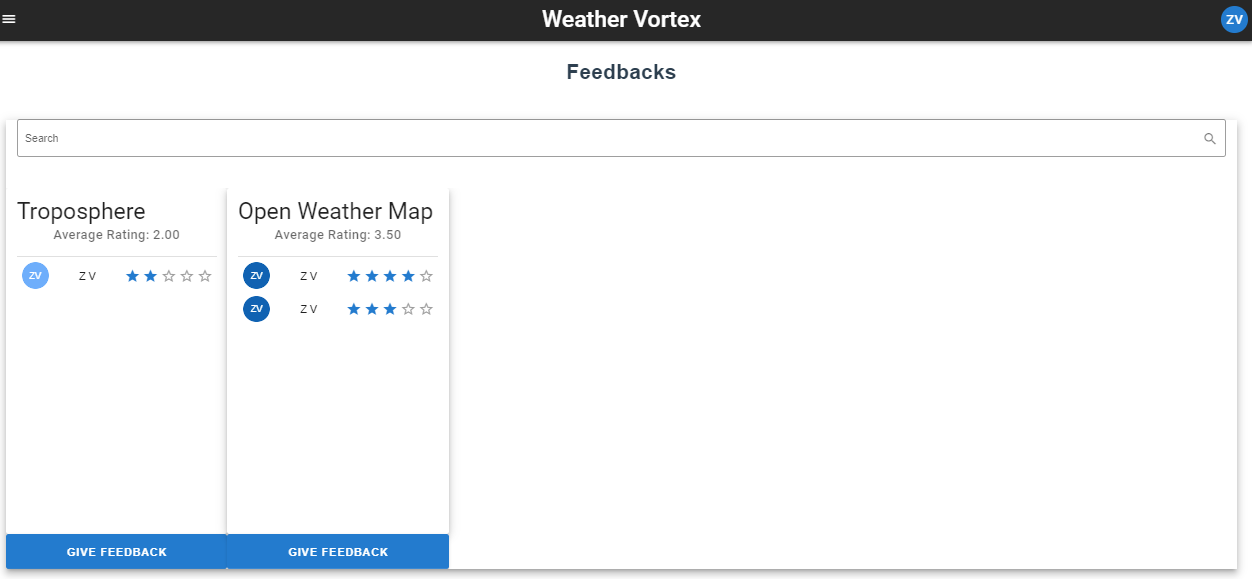
\includegraphics[width=1\textwidth]{Images/feedback.PNG}
\end{figure}
La pagina dei feedback raccoglie tutte le recensioni lasciate dagli utenti divise per provider. Anche qui è possibile ricercarne uno con l'apposita barra. Cliccando sull'icona di un utente si viene indirizzati al suo profilo pubblico. Qualora si sia autenticati
è possibile lasciare una recensione direttamente dal pulsante sottostante.

\begin{figure}[H]
    \caption{Pagina About finale}
    \label{fig:imAbout}
    \centering
    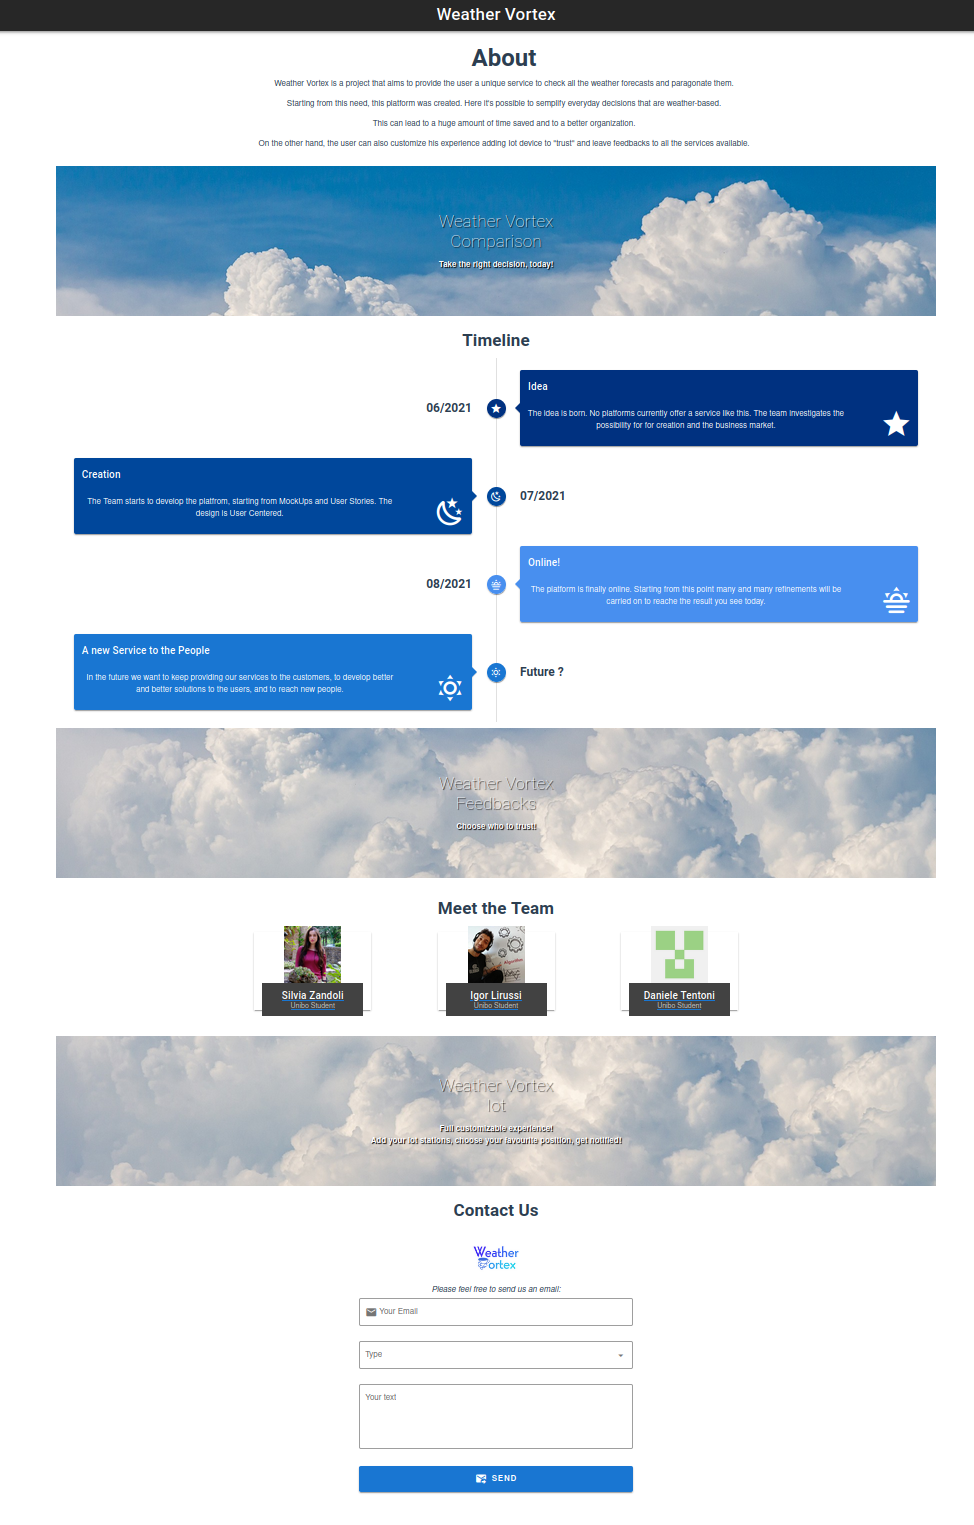
\includegraphics[width=1\textwidth]{Images/about.PNG}
\end{figure}